\chapter[Estruturação e Implementação da Gamificação da About]{Estruturação e Implementação da Gamificação da About}

Para a implementação do trabalho, os seguintes
passos foram executados, cada um é
descrito em uma subsessão: execução do teste piloto, \textit{survey} para identificação das técnicas de gamificação,
análise estatística das técnicas, construção do \textit{framework} de gamificação, escolha do objeto de gamificação,
implementação das técnicas no objeto de gamificação.

Aqui será relatado todos os passos que foram tomados para a realização do trabalho.


% \section{Planejamento}
% \label{sec:planejamento}

% \section{Definição da Gamificação}
% \label{sec:definicao_gamification}

\section{Execução do Piloto}
\label{sec:execucao_do_piloto}
Com a intenção de validar a aplicação da About, foi implementado um piloto com as suas funcionalidades
básicas. Aqui existia apenas um post, onde o administrador um da aplicação escolhe dentre temas propostos
pelos usuários, que era postado a cada três dias.
Nesta sessão iremos descrever sobre como esta implementação foi executada.

Para desenvolver e aplicar este piloto, será necessário executar um procedimento
com os seguintes passos:

\begin{enumerate}
    \item Definir tecnologia;
    \item Desenvolver solução;
    \item Implantação em produção;
    \item Aplicar \textit{marketing} da solução para um público reduzido;
    \item Manter solução;
    \item Finalizar solução.
\end{enumerate}


Primeiramente, haviam alguns pontos necessários ppara a implantação da aplicação. Assim como agilidade para colocar
em produção e desenvolvimento rápido. Estes foram os padrões seguidos para a produção do piloto:


\begin{itemize}
    \item Desenvolvimento rápido;
    \item Padrões de Design simples;
    \item Escalabilidade baixa;
    \item Os usuários não carecem de executar cadastros e logins;
    \item Suporte para questionários;
    \item Facilidade de implantação.
\end{itemize}

Assim, estes pontos foram avaliados. Desta forma, era necessário implementar um software
de alta produtividade, que entregasse a funcionalidade muito rapidamente. Assim, dados estes
pontos, a tecnologia escolhida foi o WordPress, utilizando a linguagem de programação PHP.

Esta possui vários módulos prontos, desenvolvidos pela comunidade e forneceidos de maneira
gratuita. Nestes módulos, temos componentes para questionários, design de interface já
implementados facilmente e de extrema facilidade para implantação.

Como o software é considerado pequeno, não houve nenhuma necessidade de preocupação com a
infraestrutura  do sistema e com fatores técnicos ligados à alta performace. Também não foi
necessário fazer um controle de acessos e de usuários, pois a votação seria baseada no IP
do cliente, não permitindo novos acessos daquele mesmo IP.

Escolhida a tecnologia, foi iniciada a implementação da aplicação. Esta consistiu em escolher o
módulo de enquete e o módulo de layout. Após isto, tudo estava finalizado.

Para enquetes, foi
utilizado o pacote WP-Polls, este pode ser encontrado em: \url{https://wordpress.org/plugins/wp-polls/}.

Para a implementação do layout foi utilizado o módulo Amadeus, que pode ser encontrado em:
\url{https://br.wordpress.org/themes/amadeus/}.

No âmbito da implantação foi necessário apenas comprar um servidor cloud e instalar os pacotes do WordPress
dentro deste. O código fonte da aplicação pode ser encontrado neste link:
\url{https://wordpress.org/download/}.

Implementada a solução e operando, foi necessário divulgá-la para aqueles que utilizariam o código.
Então foi criado um perfil na rede social FaceBook, onde este divulgou para todos os alunos de engenharia
de software o propósito do site, bem como cada um poderia utilizá-lo. Assim, foram feitas postagens diárias
na página falando sobre as notícias da aplicação. A comunidade em si se empolgou bastante com os novos resultados.

O perfil ganhou vários seguidores que participavam ativamente ou passivamente da plataforma, respondendo, criando e
visualizando os posts realizados no projeto piloto.

Para manter a solução, era necessário levantar enquetes para o público. Então, para manter o público interessado,
foi criado uma segunda enquete que sempre estava disponível perguntando aos usuários:

Qual seria o tema que eles desejavam ver no próximo post do piloto?

Assim, todos os temas mais pedidos pelo público era lançado e operando ao longo de dois dias para uma votação.

Por fim, foi declarado que seria finalizada a solução e que o último post seria feito. Este foi realizado para a
última votação. E assim o piloto saiu de produção.

\section{Levantamento das Técnicas de Gamificação}
\label{sec:gamifição}
Com base em uma pesquisa executada com os participantes do piloto, foi executado um levantamento das
técnicas básicas, para colocá-las frente aos objetivos estabelecidos no trabalho.

Primeiramente foi perguntado a alguns usuários que utilizaram a rede social para executar alguns
pontos relativos à impressão destes ao piloto. Detalhes sobre como estes viam as impressões passadas.
Claro que o intuito de todas as perguntas era idetificar como os usuários visualizavam dinâmicas
que envolviam gamificação dentro do piloto.

As perguntas realizadas aos usuários foram as seguintes:

\begin{quotation}
    Questão 01: Na sua opinião, o que este \textit{site} representava?
\end{quotation}

\begin{quotation}
    Questão 02: O que você acredita que motivava e levava as pessoas a utilizarem o \textit{site}?
\end{quotation}

\begin{quotation}
    Questão 03: E quanto ao contrário, o que você acredita que levava as pessoas a se desmotivarem e a não
    utilizarem mais o \textit{site}?
\end{quotation}

Assim, para estas perguntas, tivemos um total de 4 pessoas respondendo este questionário. A resposta de cada
usuário será descrita a seguir. Iremos dividir as etapas em questões. Listando assim as quatro respostas
para cada questão.


\subsection{Questão 01}
\subsubsection{Usuário 01}
A curiosidade levava as pessoas a entrarem na plataforma e descobrirem o que as
pessoas estavam falando das outras que você conhece.
\subsubsection{Usuário 02}
Era uma oportunidade de trazer a tona todos os sentimentos e sensações das pessoas
em relação as outras. Tanto relação a atitudes quanto a impressões sobre eventos
passados. Uma oportunidade de trazer visibilidade para a consequencia de uma ação
feita por aguém.
\subsubsection{Usuário 03}
Criativo
\subsubsection{Usuário 04}
Um site que surgiu na faculdade, que a princípio era um portal para relatado de
acontecimentos da faculdade UnB-FGA, onde existiam vários posts inimagináveis
de algumas pessoas. E era confirmado este relato quando você via os outros comentários
anônimos, reforçando exatamente aquele ponto. Eram comentários que a princípio ninguém
acreditaria, pois eram extremamente fortes. Chegando a chocar com os fatos
declarados.

\subsection{Questão 02}
\subsubsection{Usuário 01}
As pessoas estarem curiosas para saberem sobre segredos sobre outras, que não
são contados no cotidiano.
\subsubsection{Usuário 02}
oportunidade de Conseguir punir ações errônias para as pessoas por atitudes erradas.
Mostrando que atitudes erradas tem consequencia, expondo o autor caso ele faça
algo de ruim para aquele meio.
\subsubsection{Usuário 03}
curiosidade
\subsubsection{Usuário 04}
Você não queria ser um alvo do post da plataforma, você quer ser aquele que julga.
Então criava-se a curiosidade sobre os comentários feitos à minha pessoa e também
os comentários feitos a outras pessoas. O ambiente de 'fofoca' estimulava o ambiente.

\subsection{Questão 03}
\subsubsection{Usuário 01}
Medo de exposição de seus detalhes pessoas para demais individuos.
\subsubsection{Usuário 02}
A probabilidade de perder o controle diante da invasão de privacidade. E trazer
consequencias reais para a vida da pessoa.
\subsubsection{Usuário 03}
Falta de atualização e novidades em novos conteúdos no portal.
\subsubsection{Usuário 04}
Medo de que seu nome estivesse ali no meio da plataforma e a falta de existência
de um meio de defesa para os acusados.

Terminadas as perguntas aos usuários, foi muito claro que para todos que o que motivava
os usuários era a curiosidade, o desconhecido, a vontade de saber sobre o que
não é conhecido.

Logo, já é possível ver a presença de algumas motivações básicas de gamificação, ligadas
à curiosidade.

Mas ainda sim, esta análise qualitativa não mostrou muito sobre quais fatores
e quais motivações básicas de fato eram percebidas no piloto executado. Assim,
como planejado, foi executado um Survey, para obter resultados quantitativos sobre
o quanto cada técnica estava influenciando o procedimento de gamificação dentro
daquela aplicação. Estes passos serão descritos na próxima sessão.

\section{Survey das Técnicas}
\label{sec:gamifição}
Para apurar as técnicas capturadas no levantamento, foi executado um survey, a fim de dados para
embasar uma análise estatística.

Para este survey, foi utilizada uma escala de 0 a 5. Assim, foram apresentadas aos usuários
que fizeram o primeiro levantamento todas as técnicas de gamificação, com a sua
respectiva explicação. O usuário deveria votar e dizer o quanto esta estava presente
dentro do escopo do piloto. As técnicas utilizadas são as apresentadas na sessão
\ref{sub:an_lise_estat_stica_das_t_cnicas}.

Primeiramente, para entender qual o perfil de entrevistado no trabalho, foi elaborado
um questionário prévio para traçar seus aspéctos pessoais,
para que pudesse ser entendido qual a relação que esse tem com jogos e com dinâmicas
voltadas à gamificação. Todos estes podem ser vistos neste \href{https://docs.google.com/spreadsheets/d/1galTU00NPQKaU7GRsYOciLhD0ZzIKH9BbJWyRdC3gbs/edit?usp=sharing}{link}.


Para a elaboração desta, foi apresentado um formulário a cada usuário, solicitando
que este votasse em todas as técnicas. A tabela com o resultado está neste seguinte
\href{https://docs.google.com/spreadsheets/d/1qROpsDaz32PZtkvCvmFTrqLVLgqhHR9F-Q5rcQ_pwys/edit?usp=sharing}{link}.

Assim, com esses dados obtidos, foi possível executar os cálculos da sessão \ref{sub:implementa_o_das_t_cnicas}
e montar o framework, como apresentado no exemplo da figura \ref{fig:exoctalysis}.

Antes de executar o cálculo, foi elaborada a Tabela \ref{tab:percentual_tecnica_motivacao}
 de notas, onde é possível
observar a quantidade total possível e a quantidade de pontos feita por cada técnica.
Bem como a porcentagem que esta representa.

% Please add the following required packages to your document preamble:
% \usepackage{booktabs}
\begin{table}[]
\centering
\caption{Percentual de Técnica por Motivação Básica}
\label{tab:percentual_tecnica_motivacao}
\begin{tabular}{@{}cccc@{}}
\toprule
Motivação Básica & Pontos Totais & Pontos de Votos & Percentual \\ \midrule
1         & 68            & 140             & 48,57\%    \\
2         & 102           & 280             & 36,43\%    \\
3         & 62            & 160             & 38,75\%    \\
4         & 38            & 120             & 31,67\%    \\
5         & 93            & 200             & 46,50\%    \\
6         & 20            & 100             & 20,00\%    \\
7         & 74            & 120             & 61,67\%    \\
8         & 32            & 60              & 53,33\%    \\ \bottomrule
\end{tabular}
\end{table}

Executada esta tabela, já seria possível criar o framework de gamificação. Assim,
este finalizado pode ser visto na Figura.

\begin{figure}[h]
    \centering

    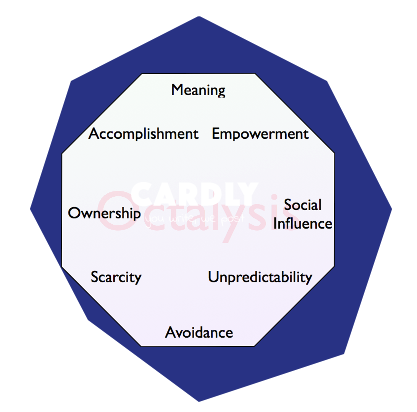
\includegraphics[width=250px, scale=1]{figuras/final_survey}
    \caption{Framework final do Survey}

    \label{fig:final_framework_octalisys}
\end{figure}

Assim, como todos estes dados, é possível iniciar um procedimento de estudo de Dados.
Todas essas análises serão feitas na próxima sessão.

\section{Análise Estatística}
\label{sec:gamifição}
Com base nestes dados, foram definidos quais as técnicas tem relação entre si para auxiliar no processo
da escolha destas para o Framework.

Todos estes estudos com base nos dados foram feitos através do resultado do survey aplicado nos usuários
da plataforma. Estes foram armazenados em uma planilha ods.

Para fazer todas essas análises, primeiramente foi necessário escolher uma ferramenta de processamento de dados.

Como a ferramenta escolhida foi a RScript, da sessão 4.4.1, iremos proceder todos os detalhes de implementação
levando em consideração essa tecnologia.


Assim, primeiramente foi feita a instalação dos pacotes. Primeiramente é analisado
se este está instalado dentro da máquina. 
Caso esteja, o projeto vai continuar o código contrário, estes serão instalados.

\lstinputlisting[language=Python, firstline=3, lastline=10]{statistics.r}

Assim que a aplicação certifica que todos estão instalados, estes são carregados
para a aplicação da seguinte maneira:

\lstinputlisting[language=Python, firstline=12, lastline=19]{statistics.r}

carregados todos os módulos, iniciamos em um processo de leitura da tabela ods.

\section{Construção do Framework}
\label{sec:gamifição}
Definidas as técnicas para a implementação, estas foram utilizadas para a construção do Framework
de Gamificação.

\section{Objeto de Gamificação}
\label{sec:gamifição}
Assim que todo o framework foi montado, possibilitou então que fossem escolhidos em quais
pontos da About seria possível aplicá-los. Esta sessão irá discutir sobre todos os pontos de escolha
dos objetos de Gamificação.

\section{Implementação das Técnicas}
\label{sec:gamifição}
Assim que todo o framework foi estabelecido e seus objetos também, foi possível implementar
na rede social todos os pontos para colocar estas técnicas em prática.
